\documentclass[11pt]{article}

\usepackage[a4paper,margin=2.5cm]{geometry}
\usepackage{amsmath,amssymb}
\usepackage{mathtools}
\usepackage{graphicx}
\graphicspath{{../assets/}}
\usepackage{float}
\usepackage{booktabs}
\usepackage{listings}
\usepackage{xcolor}
\usepackage[most]{tcolorbox}
\usepackage{hyperref}

\setcounter{MaxMatrixCols}{20}

\lstset{
    basicstyle=\ttfamily\small,
    breaklines=true,
    columns=fullflexible,
    frame=single,
    numbers=left,
    numberstyle=\tiny,
    showstringspaces=false,
}

\newtcolorbox{question}{
    colback=gray!12,
    colframe=gray!40,
    boxrule=0.5pt,
    arc=1pt,
    left=6pt,right=6pt,top=4pt,bottom=4pt,
}

\title{Image Analysis: Assignment 2}
\author{Elina Rosato}
\date{\today}

\begin{document}

\begin{titlepage}
    \centering
    \vspace*{2cm}

    {\Large Lund University\par}

    \vspace{1.5cm}

    {\large Course code: FMAN20\par}
    {\large Course name: Image Analysis\par}

    \vspace{3cm}

    {\Huge\bfseries Assignment 2\par}

    \vspace{3cm}

    {\large\itshape Elina Rosato\par}

    \vspace{2cm}

    \begin{tabular}{rl}
        Program: & MSc Program in Machine Learning, Systems and Control \\[4pt]
        Lecturer: & K. Magnus J. Oskarsson
    \end{tabular}

    \vfill

    {\large \today\par}
\end{titlepage}

\section{Filtering}

Before starting, two remarks.

The first is about the convention we use for convolution. With a $3\times3$
filter we place the centre coefficient on top of the pixel we are computing,
multiply each coefficient by the pixel underneath it and sum the products.
Two of the filters here have no centre coefficient, since $f_1$ is $3\times4$
and $f_5$ is $1\times10$ and an even-sized axis has no middle element. What
the filter actually needs is not a centre but an \emph{origin}: one
coefficient chosen to sit on the output pixel, with the others indexed as
offsets from it, so that
\[
    v(r,c) = \sum_{i,j} f(i,j)\, u(r-i,\, c-j).
\]
For an odd size the natural origin is the centre, which gives back the usual
rule. For an even size we have to pick one of the two middle coefficients, and
the two choices give the same result translated by one pixel. We use the
convention of \texttt{scipy.signal.convolve2d} with \texttt{mode='same'},
which places the origin at coefficient $\lfloor (K-1)/2\rfloor$ along a
$K$-long axis. The choice does not affect any of the conclusions below,
because a one-pixel translation cannot change whether a result is a blur, an
inversion or an edge image; it only fixes in which direction image D is
displaced and from which diagonal image E appears to be lit.

The second remark is about why two of the results are uniformly grey. If the
coefficients sum to zero, every region where the image is locally constant
maps to exactly zero, since the positive and negative contributions cancel.
The results are displayed with automatic grey-scale scaling, so the smallest
value is drawn black and the largest white, and zero therefore lands in the
middle of the scale. A flat grey area consequently does not mean that the
output was grey, it means that the output was \emph{zero}, i.e.\ that the
filter responded to nothing there.

\begin{question}
Before making the final matching, classify the filters qualitatively (for
example, smoothing, sharpening, edge/difference detection, or spatial shift)
and state what visual effect you expect from each one.
\end{question}

Three properties of a filter are enough to predict its behaviour: the sum of
the coefficients, their signs, and the symmetry of the matrix.

The sum determines the gain on constant regions. If the image takes the same
value $c$ everywhere inside the filter window, the output is $c$ times the
sum. A sum of $1$ therefore preserves brightness, a sum of $0$ maps every
constant region to zero so that only variation can produce a response, and a
negative sum maps bright to dark, which inverts the image.

The signs determine whether the filter averages or differentiates. If all
coefficients share a sign, the operation is a weighted average of the
neighbourhood, and averaging attenuates high frequencies, so the image is
smoothed. If both signs occur, the filter subtracts one part of the
neighbourhood from another, so it responds to variation rather than to
absolute intensity.

The symmetry determines what a feature looks like in the result. Rotating a
filter by $180^\circ$ pairs every coefficient with the one at the opposite
offset, and what matters is the relative sign within each pair. If the two
have opposite signs the filter is antisymmetric, so it subtracts one side of
the neighbourhood from the other, which is a directional derivative: the
response cancels wherever the image is locally symmetric and takes opposite
signs on the two sides of a feature, leaving one flank brighter than the
background and the other darker, which we read as relief. If the two have the
same sign the filter is symmetric and adds the sides instead, so nothing
cancels and both flanks are rendered identically, which gives a plain outline.

Applying this to the six filters: $f_2$ has only non-negative coefficients
summing to $1$, so it is a smoothing filter that preserves brightness, and we
expect a blurred version of the original. Filter $f_6$ has only negative
coefficients summing to $-1$, so it is the same kind of average with the sign
reversed, and we expect a slightly blurred negative. Filter $f_4$ also sums to
$1$ but combines a large positive centre coefficient with a negative surround,
which is a sharpening filter, so we expect something almost indistinguishable
from the original apart from crisper edges. Filter $f_5$ contains a single
coefficient equal to $1$, so it is a shifted unit impulse and each output
pixel is a copy of one input pixel; we expect a pure translation. Finally
$f_1$ and $f_3$ both sum to $0$, so both give a mid-grey field with only
edges drawn on it. They differ in symmetry: $f_1$ is symmetric, so we expect
plain outlines, whereas $f_3$ is antisymmetric, so we expect the embossed
appearance of a surface lit from one direction.

\begin{question}
Match each output image to the corresponding filter and motivate each match
from the structure of the filter, not only from visual similarity.
\end{question}

There are six filters and only five images, so one filter is unused.

Image A is inverted, since the dark hair has become white and the bright
background dark. Inversion is decided by the coefficient sum, and $f_6$ is the
only filter of the six whose sum is negative, so A is $f_6$. Image B is a
blurred version of the original at unchanged overall brightness, which is
exactly a non-negative weighted average with sum $1$, so B is $f_2$. Image D
has the same sharpness, contrast and brightness as the original and differs
only by a displacement, and the only filter that leaves all of those
properties untouched is the one that merely copies single pixels, so D is
$f_5$. Images C and E are the two zero-sum results and must therefore be $f_1$
and $f_3$ in some order. In C only vertical structure survives and the
horizontal strokes of the letters in ``ADELE 21'' have vanished, which matches
$f_1$; E is embossed, which matches $f_3$.

The filter left over is $f_4$, and this is consistent, since $f_4$ sharpens
and its output would look almost identical to the original image. No such
image appears among A--E: B is blurred and D is displaced.

\begin{question}
For at least two of the filters, explain how the signs, symmetry, and sum of
the filter coefficients support your interpretation.
\end{question}

For $f_6 = -\tfrac{1}{9}\mathbf{1}_{3\times3}$ all nine coefficients are equal
and negative. Because the magnitudes are equal, the filter is the ordinary
$3\times3$ box average multiplied by $-1$, so it smooths and inverts at the
same time. The sum is $-1$, which means a constant region of intensity $c$ is
mapped to $-c$. This is why A is a negative, and since no other filter has a
negative sum, no other filter could have produced it.

For $f_1$ the three rows are identical, so the matrix has rank one and is
separable:
\[
    f_1 = \frac{1}{6}
    \begin{bmatrix} 1 \\ 1 \\ 1 \end{bmatrix}
    \begin{bmatrix} 1 & -1 & -1 & 1 \end{bmatrix} .
\]
This is the key structural fact, because it decouples the two directions. In
the $y$ direction the filter is $[1,1,1]$, a plain average, and an average
cannot detect variation, it can only smooth it. The filter is therefore blind
to horizontal edges. All of its selectivity comes from the row
$[1,-1,-1,1]$, which acts along $x$ only, so only vertical structure survives.
The sum is $0$, which accounts for the grey background, and the row is
symmetric, so it behaves as a second derivative and renders each line as a
double outline rather than giving it a bright and a dark side.

For $f_3$ the sum is also $0$, so the background is grey as well, but the
symmetry is the opposite: rotating the matrix by $180^\circ$ gives its
negative. The positive coefficients lie on the upper-right side of the main
diagonal and the negative ones on the lower-left, so the filter is a
directional first derivative along the direction from the lower-left corner
towards the upper-right corner. A first derivative is signed, so an edge
facing one way is rendered brighter than the grey background and an edge
facing the other way darker. Light on one side of a feature and dark on the
other is interpreted by the visual system as a surface under directional
illumination, which is why E appears embossed.

\begin{question}
Identify one match that is especially easy to distinguish and one that is
potentially more ambiguous, and explain why.
\end{question}

The easiest match is A with $f_6$, and it can be settled from a single number.
The coefficient sum is the gain applied to constant regions, and $f_6$ is the
only filter whose sum is negative, so it is the only one capable of inverting
intensities. Image A is unambiguously inverted, so the match follows without
examining any detail.

The difficult pair is C and E, that is $f_1$ against $f_3$. They agree on the
properties that govern the overall appearance: both sum to zero, so both
produce a mid-grey field carrying only edge information, and both have small
support, so both produce a thin and faint response. At the printed size the
two images are the same kind of picture, and neither the sum nor the sign
pattern distinguishes them.

What does distinguish them is orientation selectivity and symmetry. Because
$f_1$ contains an average in the $y$ direction, its response to a purely
horizontal edge is not merely weak but identically zero.


\section{Interpolation}

The signal is $f = \begin{bmatrix}1 & 2 & 2 & 4 & 7 & 6 & 5\end{bmatrix}$,
sampled at the points $i = 1,\dots,7$.

\begin{question}
Explain what linear interpolation means. Sketch the linear interpolation
$F_{lin}(x)$ of $f$ for $1 \le x \le 7$. Is $F_{lin}(x)$ continuous? Is
$F_{lin}(x)$ differentiable?
\end{question}

Linear interpolation means joining neighbouring samples by straight line
segments. For $x$ in $[i,i+1]$, writing $t = x-i$ so that $t$ runs from $0$ to
$1$ across the interval,
\[
    F_{lin}(x) = (1-t)\,f(i) + t\,f(i+1),
\]
a weighted average of the two surrounding samples in which each weight is the
closeness to that sample.

\begin{figure}[H]
    \centering
    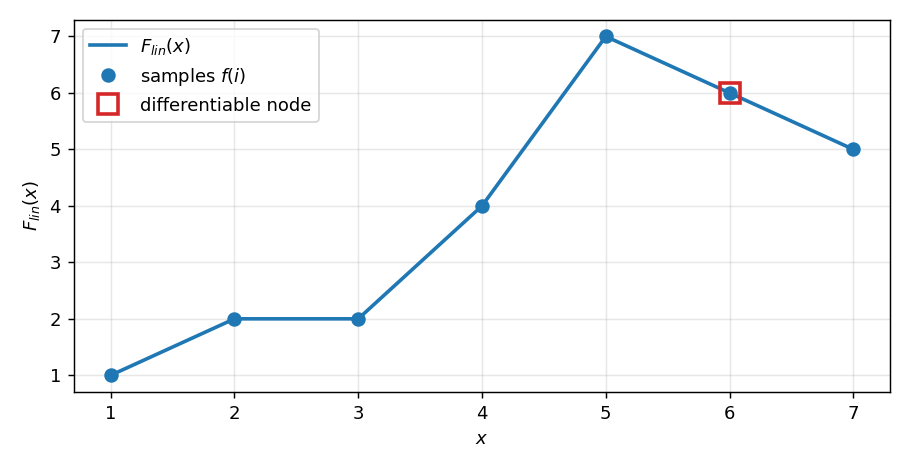
\includegraphics[width=0.75\textwidth]{interp_linear.png}
    \caption{The linear interpolation of $f$. The square marks $x=6$, the one
    interior node where the interpolant is differentiable.}
\end{figure}

It is continuous. Each piece is a polynomial, so continuity can only fail at a
node, and at $x=i$ the piece on the left ends at $f(i)$ while the piece on the
right starts at $f(i)$, so the two one-sided limits agree.

It is not differentiable everywhere. Inside an interval the interpolant is a
straight line, but at a node the one-sided derivatives are
$F_{lin}'(i^-) = f(i)-f(i-1)$ and $F_{lin}'(i^+) = f(i+1)-f(i)$, which agree
only when the data has the same difference on both sides. Since the samples
are one apart, each difference $f(i+1)-f(i)$ is exactly the slope of that
segment, and the six slopes are $+1, 0, +2, +3, -1, -1$. They disagree at
$x = 2,3,4,5$ and agree at $x=6$, where both are $-1$. Differentiability
therefore fails only at those nodes where the slope actually changes, which
depends on the data rather than on the method.

\begin{question}
Which function $g(x)$ corresponds to linear interpolation? Give the function
$g(x)$ for $-4 \le x \le 4$.
\end{question}

It is the triangle, or hat, function
\[
    g(x) = \begin{cases}
        1 - |x| & \text{if } |x| < 1, \\
        0 & \text{otherwise},
    \end{cases}
\]
so on $-4 \le x \le 4$ it is the triangle on $(-1,1)$ and zero elsewhere.

To check it, take $x$ in $[i,i+1]$ and put $t = x-i$. Every term of
$F_g(x) = \sum_k g(x-k) f(k)$ vanishes except $k=i$ and $k=i+1$, since all
other arguments exceed $1$ in absolute value. The two surviving weights are
$g(t) = 1-t$ and $g(t-1) = t$, giving $(1-t)f(i) + t f(i+1)$, which is
$F_{lin}$. Two properties matter for the comparison later: $g(0)=1$ with
$g(k)=0$ at every other integer, which makes the curve pass through the data,
and support $[-1,1]$, so only two samples affect any value.

\begin{figure}[H]
    \centering
    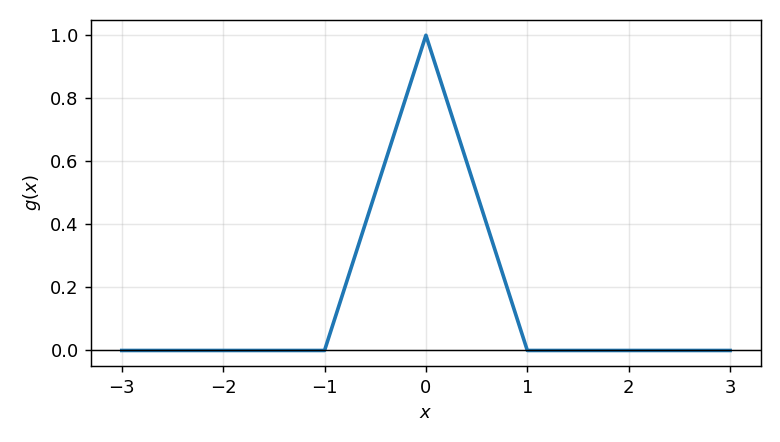
\includegraphics[width=0.6\textwidth]{interp_kernel_tri.png}
    \caption{The triangle kernel, the $g$ that reproduces linear
    interpolation.}
\end{figure}

\begin{question}
Let $g(x) = \tfrac{6}{7}(1-|x|^2)$ for $|x| \le 1$,
$g(x) = -\tfrac{6}{7}(|x|^3 - 5|x|^2 + 8|x| - 4)$ for $1 < |x| \le 2$, and
$g(x) = 0$ for $|x| > 2$. Plot $g(x)$ for $-3 \le x \le 3$. Plot the
interpolation $F_g$ of $f$ using this $g$, for $1 \le x \le 7$. Is $F_g(x)$
continuous? Is $F_g(x)$ differentiable?
\end{question}

\begin{figure}[H]
    \centering
    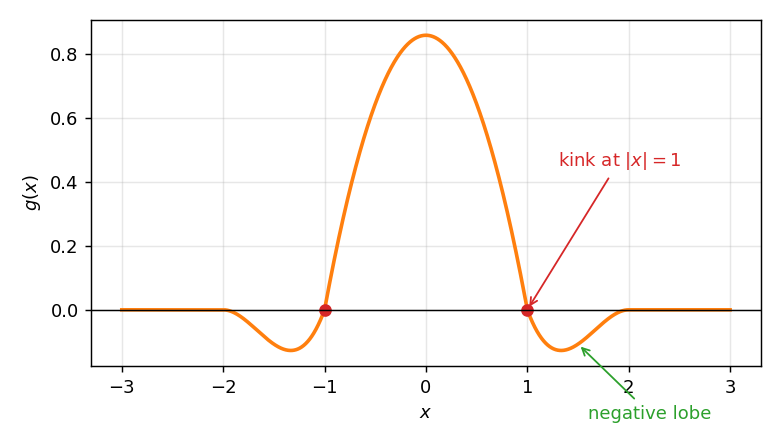
\includegraphics[width=0.49\textwidth]{interp_kernel_cub.png}
    \hfill
    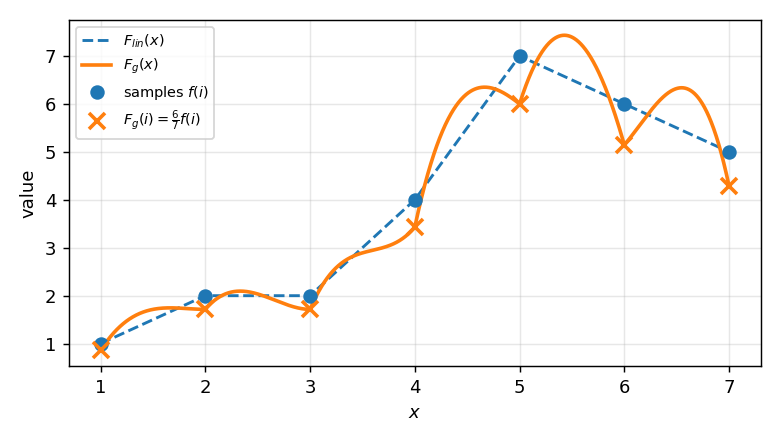
\includegraphics[width=0.49\textwidth]{interp_Fg.png}
    \caption{Left: the kernel $g$, with the kink at $|x|=1$ and the negative
    side lobes marked. Right: the interpolation $F_g$ (solid) with the linear
    interpolation (dashed) and the samples; the crosses show that $F_g$ passes
    not through $f(i)$ but through $\tfrac{6}{7} f(i)$.}
    \label{fig:Fg}
\end{figure}

Since the answers depend on the behaviour of $g$ at its joining points, we
inspect those first. Writing $s = |x|$, the two joins are at $s=1$ and $s=2$,
and both pieces vanish at each of them, so $g$ is continuous. Differentiating
the pieces as given, $\tfrac{6}{7}(1-s^2)$ has derivative $-\tfrac{12s}{7}$
and $-\tfrac{6}{7}(s^3-5s^2+8s-4)$ has derivative
$-\tfrac{6}{7}(3s^2-10s+8)$, so

\begin{table}[H]
    \centering
    \begin{tabular}{lccl}
        \toprule
        join & from the left & from the right & \\
        \midrule
        $s=1$ & $-12/7$ & $-6/7$ & kink \\
        $s=2$ & $0$ & $0$ & differentiable \\
        \bottomrule
    \end{tabular}
    \caption{One-sided derivatives of $g$ at its joining points.}
\end{table}

So $g$ is continuous everywhere and differentiable everywhere except at
$|x|=1$, where $g'$ jumps by $6/7$. (The join at $s=2$ is smooth because the
cubic factors as $(s-1)(s-2)^2$: the double root makes both $g$ and $g'$
vanish there, whereas the simple root at $s=1$ makes only $g$ vanish.)

These properties carry over to $F_g = \sum_{i=1}^{7} g(x-i) f(i)$, which is a
finite sum of shifted, scaled copies of $g$. A finite sum of continuous
functions is continuous, so \textbf{$F_g$ is continuous everywhere}.

For differentiability, the term $g(x-i)$ can only be non-differentiable where
its argument reaches $\pm1$, that is at $x = i \pm 1$, so all possible kinks
of $F_g$ sit at integers and everywhere else $F_g$ is a finite sum of
differentiable functions. At a node $x=m$ exactly two terms kink, the ones
with $i = m-1$ and $i = m+1$, whose arguments pass through $+1$ and $-1$. The
jump in $g'$ is $6/7$ at both places, since $g$ is even and therefore $g'$ is
odd, so
\[
    F_g'(m^+) - F_g'(m^-) = \tfrac{6}{7}\big[\,f(m-1) + f(m+1)\,\big].
\]
At $x=4$, for instance, only the terms $i=3$ and $i=5$ kink and the jump is
$\tfrac{6}{7}(2+7) = 54/7 \approx 7.71$. All samples are positive, so the
expression is never zero and \textbf{$F_g$ is not differentiable at any
interior node}. The jumps at $x=2,\dots,6$ are $18/7, 36/7, 54/7, 60/7$ and
$72/7$, and one-sided difference quotients computed numerically reproduce
these to four decimals.

Finally, note that $g(0) = \tfrac{6}{7}$ rather than $1$, while
$g(\pm1)=g(\pm2)=0$. At a sample point only one term survives, so
$F_g(i) = \tfrac{6}{7} f(i)$ and the curve misses every data point by that
factor, as the crosses in Figure~\ref{fig:Fg} show. Strictly this $g$ is a
smoothing kernel rather than an interpolating one; the factor $6/7$ normalises
$\int g = 1$ instead of $g(0)=1$.

\begin{question}
Compare the interpolation obtained with this $g$ with the linear
interpolation: comment on locality, smoothness, and how values between the
samples are influenced by neighbouring samples.
\end{question}

\textbf{Locality.} The triangle kernel has support $[-1,1]$, so $F_{lin}(x)$
depends on the two samples bracketing $x$. The kernel $g$ has support
$[-2,2]$, so $F_g(x)$ generally depends on four: at $x=3.5$ the samples
$f(2),\dots,f(5)$ all contribute, against only $f(3)$ and $f(4)$ for linear
interpolation. Wider support means a local error in the data spreads further.

\textbf{Smoothness.} Between the nodes $F_g$ is a cubic and therefore curved,
so it looks smoother than the straight segments of $F_{lin}$, but at the nodes
both are only continuous. $F_{lin}$ kinks wherever the data changes slope,
while $F_g$ kinks at every node, including $x=6$ where $F_{lin}$ does not. By
the strict criterion the cubic construction is thus the less regular of the
two here: what it buys is curvature between the nodes, not differentiability
at them.

\textbf{Influence of neighbouring samples.} The decisive property is the sign
of the kernel. The triangle kernel is non-negative with weights summing to
$1$, so $F_{lin}$ is a convex combination of two data values and can never
leave the range of the data. The kernel $g$ is negative on $1 < |x| < 2$, so
the outer samples enter with negative weight and push the curve away from
them. Two consequences are visible in Figure~\ref{fig:Fg}. The data is flat on
$[2,3]$, where $f(2)=f(3)=2$, and $F_{lin}$ is correspondingly exactly flat,
but $F_g$ bulges to $2.095$ at $x \approx 2.33$ because $f(1)$ and $f(4)$ act
through the negative lobes. And although the largest sample is $f(5)=7$,
$F_g$ reaches $7.43$ at $x \approx 5.43$, overshooting the range of the data,
which non-negative weights cannot do. This overshoot is the one-dimensional
version of the bright and dark fringes a sharpening filter produces along an
edge.


\section{Classification using Nearest Neighbour and Bayes theorem}

The measurements are

\begin{table}[H]
    \centering
    \begin{tabular}{lccccccc}
        \toprule
        Class 1 & 0.4003 & 0.3985 & 0.3998 & 0.3997 & 0.4015 & 0.3995 & 0.3991 \\
        Class 2 & 0.2554 & 0.3139 & 0.2627 & 0.3802 & 0.3247 & 0.3360 & 0.2974 \\
        Class 3 & 0.5632 & 0.7687 & 0.0524 & 0.7586 & 0.4443 & 0.5505 & 0.6469 \\
        \bottomrule
    \end{tabular}
\end{table}

Before computing anything it is worth looking at how the three groups sit on
the axis, since that already predicts where the difficulty will be. Alongside
the measurements we also have the Gaussian model of Section~3.2, which
specifies the class means and standard deviations as $m_1 = 0.40$,
$\sigma_1 = 0.01$; $m_2 = 0.32$, $\sigma_2 = 0.05$; and $m_3 = 0.55$,
$\sigma_3 = 0.2$. These are given as known parameters rather than estimated
from the data, and they are close to but not identical with what we would
estimate from the measurements themselves. Using
$\hat{\mu} = \frac{1}{N}\sum_i x_i$ and
$\hat{\sigma}^2 = \frac{1}{N}\sum_i (x_i - \hat{\mu})^2$, the seven samples of
each class give $\hat{\mu} = 0.3998,\ 0.3100,\ 0.5407$ and
$\hat{\sigma} = 0.0009,\ 0.0400,\ 0.2265$.

Class 1 is extraordinarily concentrated: all seven values lie between $0.3985$
and $0.4015$, a span of $0.0030$. Class 2 is moderately spread, from $0.2554$
to $0.3802$ about its mean of $0.32$. Class 3 is spread very widely, from
$0.0524$ to $0.7687$ with $\sigma_3 = 0.2$, so its samples straddle both of
the other two classes. We therefore expect class 1 to
be the easiest, since it occupies a tiny interval that no other class
concentrates on, and class 3 to be the hardest, since some of its samples fall
closer to the other two classes than to the bulk of their own. Class 2 should
be intermediate, with its upper tail reaching towards class 1.

\subsection{Nearest Neighbours}

\begin{question}
Use nearest neighbour classification. Assume that the first four measurements
in each class are used for training and the last three for testing. How many
measurements will be correctly classified?
\end{question}

With four training and three test samples per class there are twelve training
points and nine test points. Each test point is given the label of the
training point nearest to it. \textbf{Eight of the nine are correct.} All
three test samples of class 1 and all three of class 2 are classified
correctly; of class 3, two are correct and $x = 0.4443$ is not.

As a worked example, take that failing point. Its distance to the nearest
training sample of each class is

\begin{table}[H]
    \centering
    \begin{tabular}{lcc}
        \toprule
        & nearest training sample & distance \\
        \midrule
        class 1 & $0.4003$ & $\mathbf{0.0440}$ \\
        class 2 & $0.3802$ & $0.0641$ \\
        class 3 & $0.5632$ & $0.1189$ \\
        \bottomrule
    \end{tabular}
\end{table}

The smallest distance belongs to class 1, so the point is assigned to class 1
although it truly belongs to class 3. The error is easy to explain from the
training data. The four training samples of class 3 are $0.0524$, $0.5632$,
$0.7586$ and $0.7687$, which leaves a wide empty stretch between $0.05$ and
$0.56$, and $0.4443$ falls inside it. The four training samples of class 1, by
contrast, all lie within $0.002$ of $0.4$, so any point in that neighbourhood
is close to one of them. Nearest neighbour compares only raw distances to
individual samples, so a sparsely sampled class with a gap loses to a densely
sampled class nearby.

\subsection{Gaussian distributions}

\begin{question}
Assume that the measurements have normal distribution with known parameters
(expected value $m_i$ and variance $\sigma^2$): $m_1 = 0.4$,
$\sigma_1 = 0.01$; $m_2 = 0.32$, $\sigma_2 = 0.05$; $m_3 = 0.55$,
$\sigma_3 = 0.2$. All classes are equally likely to occur. What is the maximum
a posteriori classification of a measured $x$? How many measurements are
correctly classified?
\end{question}

The rule is to pick the class with the largest posterior,
\[
    \hat{\jmath} = \arg\max_k P(Y = k \mid x),
\]
and Bayes' theorem rewrites that posterior in terms of quantities we can
actually compute,
\[
    P(Y = k \mid x) = \frac{f_X(x \mid Y = k)\, P(Y = k)}{f_X(x)},
    \qquad
    f_X(x) = \sum_j f_X(x \mid Y = j)\, P(Y = j).
\]
The denominator $f_X(x)$ does not depend on $k$, so it is one and the same
number for all three classes and cannot affect which posterior is largest;
only the numerators need to be compared. Here the classes are in addition
equally likely, $P(Y=k) = 1/3$, so the prior is a common factor as well and
also drops out. What remains is to choose the largest likelihood
\[
    f_X(x \mid Y = k)
    = \frac{1}{\sigma_k \sqrt{2\pi}}
      \exp\!\left(-\frac{(x - m_k)^2}{2\sigma_k^2}\right).
\]
No measurements were used for training, so all twenty-one are classified.
\textbf{Twenty of the twenty-one are correct}: classes 1 and 3 are classified
perfectly and the single error is $x = 0.3802$, a class 2 sample assigned to
class 1.

For that point the three likelihoods are
\begin{align*}
    f_X(x \mid Y = 1) &= \frac{1}{0.01\sqrt{2\pi}}\,e^{-1.98^2/2}
      = 39.89 \times 0.1408 = 5.618, \\
    f_X(x \mid Y = 2) &= \frac{1}{0.05\sqrt{2\pi}}\,e^{-1.204^2/2}
      = 7.98 \times 0.4844 = 3.865, \\
    f_X(x \mid Y = 3) &= \frac{1}{0.20\sqrt{2\pi}}\,e^{-0.849^2/2}
      = 1.99 \times 0.6974 = 1.391,
\end{align*}
so class 1 wins. This deserves a comment, because measured in units of each
class's own standard deviation the point is $1.98\sigma$ away from class 1 but
only $1.20\sigma$ away from class 2, so counting standard deviations alone
would have favoured class 2. Taking logarithms,
\[
    \ln f_X(x \mid Y = k) = -\frac{(x-m_k)^2}{2\sigma_k^2} - \ln \sigma_k
    + \text{const},
\]
which shows that the decision is not made on the number of standard deviations
alone: the term $-\ln \sigma_k$ gives a bonus to narrow classes. Class 1 is
five times narrower than class 2, so its density is five times taller at its
peak, and that is enough to overcome the extra distance.

Scanning the winning class across the axis gives the decision regions

\begin{table}[H]
    \centering
    \begin{tabular}{lc}
        \toprule
        region & decision \\
        \midrule
        $x < 0.1990$ & class 3 \\
        $0.1990 < x < 0.3786$ & class 2 \\
        $0.3786 < x < 0.4253$ & class 1 \\
        $x > 0.4253$ & class 3 \\
        \bottomrule
    \end{tabular}
    \caption{MAP decision regions for equal priors.}
\end{table}

Class 1 owns only the narrow window $[0.3786, 0.4253]$, of width $0.047$,
because its small $\sigma$ makes its density collapse quickly away from
$0.4$; and because class 3 is so broad it claims everything far from the other
two means, on both sides.

\begin{figure}[H]
    \centering
    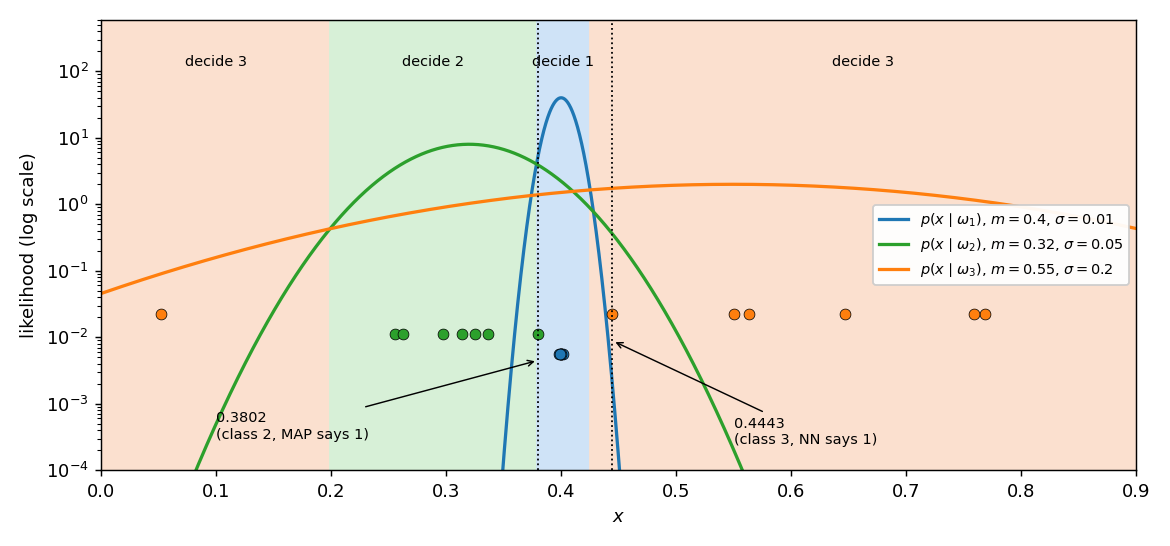
\includegraphics[width=\textwidth]{classification.png}
    \caption{The three class likelihoods on a logarithmic scale, with the MAP
    decision regions shaded and the measurements shown as dots. The two
    misclassified values are marked.}
    \label{fig:classification}
\end{figure}

\subsection*{Comparison of the two classifiers}

Our predictions were right. Class 1 is classified perfectly by both methods,
and the two errors fall in classes 2 and 3, the ones we expected to be harder.
Each error has its own cause. Nearest neighbour misses $0.4443$ because the
four training samples of class 3 leave a wide gap between $0.05$ and $0.56$
and that point falls inside it. MAP misses $0.3802$ because it is the most
extreme sample of class 2 and reaches into the narrow window belonging to
class 1.

The two methods can disagree about the same value because they measure
closeness in different ways. Nearest neighbour uses the plain distance to the
closest training sample. The Gaussian model divides that distance by the
standard deviation of the class, so it asks how \emph{surprising} the distance
is rather than how large it is. For $x = 0.4443$ the plain distances are
$0.0440$ to class 1 and $0.1189$ to class 3, so nearest neighbour picks class
1. Measured in standard deviations the same point is $4.43\sigma_1$ from $m_1$
but only $0.53\sigma_3$ from $m_3$, so MAP picks class 3 and is right. Nearest
neighbour has no way of knowing that a deviation of $0.044$ is ordinary for
class 3 and impossible for class 1.

If the classes were not equally likely the priors would no longer cancel, and
we would maximise $\ln f_X(x \mid Y=k) + \ln P(Y=k)$. Each class then gets a
fixed bonus $\ln P(Y=k)$ that does not depend on $x$, so the curves keep their
shape but every boundary moves towards the less likely class. A class with a
small prior needs stronger evidence from the measurement before it is chosen.


\section{Image Classification}

A scene is one of three possible $2\times2$ binary images, with the a priori
probabilities
\[
    Y = 1:\ \begin{bmatrix} 0 & 1 \\ 1 & 0 \end{bmatrix} \ \ \tfrac{1}{4},
    \qquad
    Y = 2:\ \begin{bmatrix} 1 & 0 \\ 0 & 1 \end{bmatrix} \ \ \tfrac{1}{2},
    \qquad
    Y = 3:\ \begin{bmatrix} 1 & 1 \\ 1 & 0 \end{bmatrix} \ \ \tfrac{1}{4}.
\]
One of them has been sent through a noisy channel that flips each pixel
independently with probability $\epsilon$, and the image we actually observe
is
\[
    x = \begin{bmatrix} 0 & 1 \\ 1 & 1 \end{bmatrix}.
\]

\begin{question}
Using Bayes theorem, calculate the posterior probabilities and the MAP
estimate of the scene for (a) $\epsilon = 10\%$ and (b) $\epsilon = 50\%$.
Show the answers in percentages or percentage decimals.
\end{question}

Since the noise acts on each pixel separately, the probability of seeing the
whole image is the product of the probabilities of seeing each of its four
pixels,
\[
    P(x \mid Y=k) = \prod_{j=1}^{4} P(x_j \mid Y=k, \text{pixel } j),
\]
and each pixel contributes only one of two numbers: $1-\epsilon$ if it agrees
with the candidate scene, because then it came through unchanged, and
$\epsilon$ if it disagrees, because then it must have been flipped. If the
scene disagrees with the observed image in $k$ of the four positions we
therefore get
\[
    P(x \mid Y=k) = \epsilon^{k}\,(1-\epsilon)^{4-k}.
\]
Only the \emph{number} of disagreements matters, not which pixels they are,
because the flip probability is the same in both directions. Counting them by
reading the images in the order top-left, top-right, bottom-left,
bottom-right, where $x = (0,1,1,1)$:

\begin{table}[H]
    \centering
    \begin{tabular}{lcccl}
        \toprule
        scene & pixels & prior $P(Y=k)$ & mismatches $k$ & likelihood \\
        \midrule
        $Y=1$ & $(0,1,1,0)$ & $1/4$ & $1$ & $\epsilon(1-\epsilon)^3$ \\
        $Y=2$ & $(1,0,0,1)$ & $1/2$ & $3$ & $\epsilon^3(1-\epsilon)$ \\
        $Y=3$ & $(1,1,1,0)$ & $1/4$ & $2$ & $\epsilon^2(1-\epsilon)^2$ \\
        \bottomrule
    \end{tabular}
\end{table}

Bayes' theorem then gives
\[
    P(Y=k \mid x) = \frac{P(x \mid Y=k)\,P(Y=k)}{P(x)},
    \qquad
    P(x) = \sum_{j} P(x \mid Y=j)\,P(Y=j),
\]
so we compute the three products $P(x \mid Y=k) P(Y=k)$ and divide each by
their sum.

\paragraph{(a) $\epsilon = 10\%$.}
The three products are
\[
    \tfrac{1}{4}(0.1)(0.9)^3 = 0.018225,
    \qquad
    \tfrac{1}{2}(0.1)^3(0.9) = 0.000450,
    \qquad
    \tfrac{1}{4}(0.1)^2(0.9)^2 = 0.002025,
\]
which sum to $P(x) = 0.020700$. Dividing:

\begin{table}[H]
    \centering
    \begin{tabular}{lccc}
        \toprule
        & $Y=1$ & $Y=2$ & $Y=3$ \\
        \midrule
        prior & $25\%$ & $50\%$ & $25\%$ \\
        posterior & $\mathbf{88.04\%}$ & $2.17\%$ & $9.78\%$ \\
        \bottomrule
    \end{tabular}
    \caption{Posteriors for $\epsilon = 10\%$; exactly $81/92$, $1/46$ and
    $9/92$.}
\end{table}

The MAP estimate is scene 1. Notice that this overturns the prior: scene 2 was
the most likely one before we looked, with $50\%$, but it drops to $2\%$,
because for scene 2 to have produced this image three of the four pixels would
have had to flip, and at $\epsilon = 10\%$ that is very unlikely. Scene 1
needs only one flip, so it rises from $25\%$ to $88\%$.

\paragraph{(b) $\epsilon = 50\%$.}
Now $\epsilon = 1 - \epsilon = 0.5$, so
\[
    P(x \mid Y=k) = (0.5)^{k}(0.5)^{4-k} = (0.5)^4 = \tfrac{1}{16}
\]
for every scene: the number of mismatches cancels out. All three likelihoods
are equal, so they are a common factor and drop out of Bayes' theorem, leaving

\begin{table}[H]
    \centering
    \begin{tabular}{lccc}
        \toprule
        & $Y=1$ & $Y=2$ & $Y=3$ \\
        \midrule
        prior & $25\%$ & $50\%$ & $25\%$ \\
        posterior & $25\%$ & $\mathbf{50\%}$ & $25\%$ \\
        \bottomrule
    \end{tabular}
    \caption{Posteriors for $\epsilon = 50\%$: identical to the priors.}
\end{table}

The MAP estimate is scene 2, which is simply the scene that was most likely
beforehand.

\paragraph{Comparing the two noise levels.}
What decides the balance is the ratio $\epsilon/(1-\epsilon)$, which we can
call the price of one mismatch. If two scenes differ by one extra mismatch,
their likelihoods differ by exactly this factor. At $\epsilon = 10\%$ the
ratio is $1/9$, so every extra mismatch makes a scene nine times less
plausible and the observed image easily outweighs the priors. At
$\epsilon = 50\%$ the ratio is $1$, so mismatches cost nothing at all and the
priors are left to decide on their own. Between the two extremes the answer
switches over: scenes 1 and 2 are equally good when
$\tfrac{1}{4}\epsilon(1-\epsilon)^3 = \tfrac{1}{2}\epsilon^3(1-\epsilon)$,
that is when $(1-\epsilon)^2 = 2\epsilon^2$, which gives
\[
    \epsilon = \frac{1}{1+\sqrt{2}} = \sqrt{2}-1 \approx 0.414 .
\]
Below that noise level the evidence wins and we answer scene 1; above it the
prior wins and we answer scene 2.

\begin{figure}[H]
    \centering
    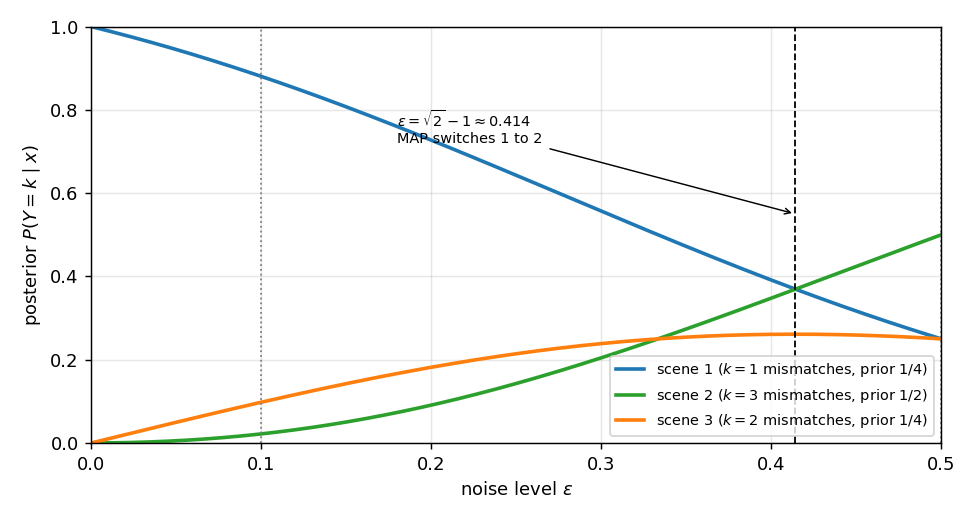
\includegraphics[width=0.8\textwidth]{image_classification.png}
    \caption{The three posteriors as functions of the noise level. At
    $\epsilon = 0$ the observation decides completely and scene 1 has
    probability $1$; as $\epsilon$ grows the three curves move towards the
    priors $25\%$, $50\%$, $25\%$, which they reach at $\epsilon = 0.5$.}
\end{figure}

\paragraph{What $\epsilon = 50\%$ means.}
At this noise level every pixel is an independent coin toss, so any observed
image is equally likely no matter which scene was sent. The observation
therefore carries no information about the scene at all: looking at the image
teaches us nothing, and the posterior is exactly what we believed before
looking.

It is worth adding that $\epsilon = 50\%$ is the \emph{only} noise level with
this property. A noise level above $50\%$ would be informative again, because
then the pixels would be reliably wrong rather than random and we could
recover the scene by inverting them. At $\epsilon = 90\%$, for example, the
posterior of scene 2 is $94.2\%$, since a scene that disagrees with the
observation in three of its four pixels is exactly what we expect to see when
most pixels have been flipped.



\section{Line Classification}

The scene is a binary $4\times4$ image which is white everywhere except for
one fully black column, and every pixel is observed wrongly with probability
$\epsilon = 0.2$ in both directions. There are four possible scenes, one for
each column, and their a priori probabilities are
\[
    P(Y=1) = 0.3, \qquad P(Y=2) = 0.2, \qquad P(Y=3) = 0.2,
    \qquad P(Y=4) = 0.3,
\]
so the outer columns are more likely than the inner ones. In the observed
image the black pixels sit at positions $(1,1)$, $(2,2)$, $(3,3)$ and $(4,2)$,
writing $(\text{row},\text{column})$.

\begin{question}
Calculate the maximum a posteriori estimation of the given image when
$\epsilon = 0.2$.
\end{question}

Before computing, it is worth guessing the answer from the picture alone.
Column 2 contains two of the four observed black pixels, columns 1 and 3
contain one each, and column 4 contains none, so we expect column 2 to be the
best candidate, columns 1 and 3 to be clearly worse, and column 4 to be worst.
We also expect columns 1 and 3 to be close to each other, since the pixel
evidence treats them alike.

The likelihood is built exactly as in the previous section. The pixels are
independent, and each one contributes $1-\epsilon$ if it matches the candidate
scene and $\epsilon$ if it does not, so a candidate that disagrees with the
observation in $k$ of the sixteen pixels has
\[
    P(x \mid Y=c) = \epsilon^{k}\,(1-\epsilon)^{16-k}.
\]
Counting the disagreements for each candidate gives $k = 6, 4, 6, 8$, as
marked in Figure~\ref{fig:line}. Bayes' theorem then gives
\[
    P(Y=c \mid x) = \frac{P(x \mid Y=c)\,P(Y=c)}{P(x)},
    \qquad
    P(x) = \sum_{j} P(x \mid Y=j)\,P(Y=j).
\]
For column 2, for example,
\begin{align*}
    P(x \mid Y=2) &= 0.2^4 \cdot 0.8^{12} = 1.0995 \times 10^{-4}, \\
    P(x \mid Y=2)\,P(Y=2) &= 0.2 \cdot 1.0995 \times 10^{-4}
      = 2.1990 \times 10^{-5}.
\end{align*}
Doing the same for all four and dividing by their sum
$P(x) = 2.5555 \times 10^{-5}$:

\begin{table}[H]
    \centering
    \begin{tabular}{ccccc}
        \toprule
        column $c$ & prior $P(Y=c)$ & mismatches $k$
        & $P(x\mid Y=c)P(Y=c)$ & posterior \\
        \midrule
        1 & $0.3$ & $6$ & $2.0616\times10^{-6}$ & $8.07\%$ \\
        2 & $0.2$ & $4$ & $2.1990\times10^{-5}$ & $\mathbf{86.05\%}$ \\
        3 & $0.2$ & $6$ & $1.3744\times10^{-6}$ & $5.38\%$ \\
        4 & $0.3$ & $8$ & $1.2885\times10^{-7}$ & $0.50\%$ \\
        \bottomrule
    \end{tabular}
    \caption{Posterior probabilities of the four line positions for
    $\epsilon = 0.2$.}
\end{table}

The MAP estimate is a line in \textbf{column 2}, and the ranking
$2 > 1 > 3 > 4$ is exactly the one we predicted from the picture.

\begin{figure}[H]
    \centering
    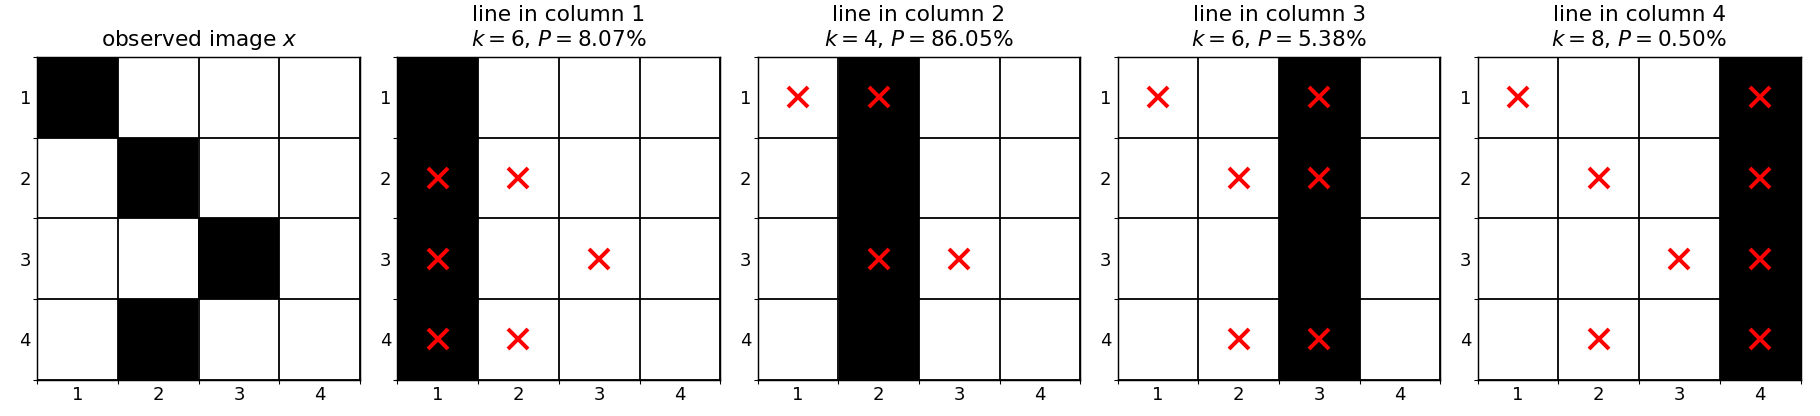
\includegraphics[width=\textwidth]{line_classification.png}
    \caption{The observed image and the four candidate scenes. Red crosses
    mark the pixels where a candidate disagrees with the observation.}
    \label{fig:line}
\end{figure}

\paragraph{Evidence for and against two candidates.}
For column 2 the evidence in favour is the pair of black pixels at $(2,2)$ and
$(4,2)$, which are exactly where the line should be. The evidence against is
of two kinds: the pixels $(1,2)$ and $(3,2)$ are white although the line
should make them black, and the pixels $(1,1)$ and $(3,3)$ are black although
they lie outside the line and should be white. That is four disagreements in
total, fewer than any other candidate.

For column 4 there is no evidence in favour at all, since none of the observed
black pixels lies in that column. Against it, all four pixels of column 4 are
white where the line should have made them black, and all four observed black
pixels are outside the column and should have been white. This gives eight
disagreements, which is the worst score of the four candidates and explains
its posterior of only $0.50\%$ despite its high prior.

\paragraph{The effect of the unequal priors.}
The priors and the pixel evidence point at different candidates here. The
priors favour the outer columns 1 and 4 with $0.3$ each, while the evidence
favours column 2, which has the fewest disagreements. The evidence wins, and
we can see by how much. Column 2 has two disagreements fewer than column 1,
and since each disagreement costs a factor $\epsilon/(1-\epsilon) = 0.25$, the
likelihood of column 2 is $4^2 = 16$ times larger. The prior works the other
way but only by a factor $0.2/0.3 = 2/3$, so the posterior ratio is
$16 \cdot \tfrac{2}{3} \approx 10.7$, which matches
$86.05/8.07$ from the table. Two extra matching pixels are simply worth far
more here than the prior preference for an outer column.

The priors are not irrelevant, though, and there is one place where they
decide everything. Columns 1 and 3 both disagree with the observation in six
pixels, so their likelihoods are identical and the pixel evidence cannot
separate them at all. What separates them is only the prior, and indeed their
posteriors stand in the ratio $8.07/5.38 = 1.50$, which is exactly
$0.3/0.2$. The prior acts as a tie-breaker when the image alone is not
informative, but it is easily overruled when the image is.



\section{Character Classification}

An image of $5\times3$ pixels shows one of three characters, with a priori
probabilities
\[
    P(Y=\text{`B'}) = 0.30, \qquad P(Y=\text{`0'}) = 0.45,
    \qquad P(Y=\text{`8'}) = 0.25 .
\]
The noise is different from the previous two sections, because it is no longer
symmetric: a truly white pixel is measured as black with probability $0.35$,
while a truly black pixel is measured as white with probability $0.2$. Writing
the four cases out,
\[
    \begin{array}{lcl}
        P(\text{white} \mid \text{truly white}) = 0.65, & \qquad &
        P(\text{black} \mid \text{truly white}) = 0.35, \\[2pt]
        P(\text{white} \mid \text{truly black}) = 0.20, & \qquad &
        P(\text{black} \mid \text{truly black}) = 0.80 .
    \end{array}
\]

\begin{question}
How should the image $x$ be classified using maximum a posteriori
probabilities (MAP) in the classification criterion?
\end{question}

As before the pixels are independent, so the likelihood of the whole image is
the product of fifteen single-pixel probabilities, each read off the table
above according to what the template says and what we observed. The important
difference from Sections~4 and~5 is that we can no longer just count
mismatches. There the two kinds of error had the same probability, so only the
total number mattered; here a mismatch on a white template pixel contributes
$0.35$ while a mismatch on a black template pixel contributes $0.20$, so the
same number of mismatches can give quite different likelihoods depending on
which kind they are. Mismatching a black pixel is $0.35/0.20 = 1.75$ times
more damaging than mismatching a white one. We therefore sort the fifteen
pixels into four groups and write
\[
    P(x \mid Y=k) = 0.65^{a}\cdot 0.35^{b}\cdot 0.20^{c}\cdot 0.80^{d},
\]
where $a$ counts the pixels that are white in the template and white in $x$,
$b$ white in the template but black in $x$, $c$ black in the template but
white in $x$, and $d$ black in both.

\begin{figure}[H]
    \centering
    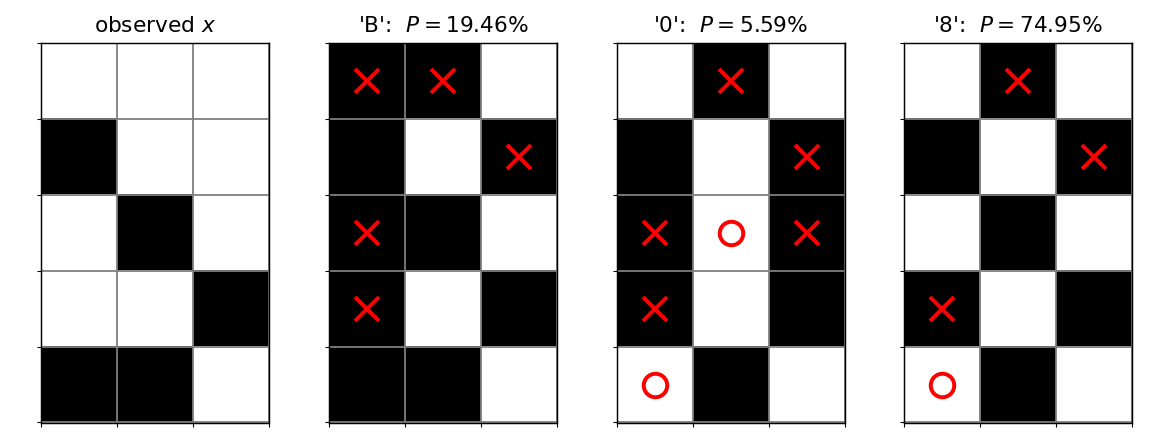
\includegraphics[width=0.85\textwidth]{character_classification.png}
    \caption{The observed image and the three templates. A cross marks a black
    template pixel observed as white (contributing $0.20$), a circle marks a
    white template pixel observed as black (contributing $0.35$).}
    \label{fig:char}
\end{figure}

Counting the four groups from Figure~\ref{fig:char} and multiplying by the
priors gives

\begin{table}[H]
    \centering
    \begin{tabular}{lccccccc}
        \toprule
        & $a$ & $b$ & $c$ & $d$ & $P(x \mid Y=k)$ & $P(x\mid Y=k)P(Y=k)$
        & posterior \\
        & $(0.65)$ & $(0.35)$ & $(0.20)$ & $(0.80)$ & & & \\
        \midrule
        `B' & 5 & 0 & 5 & 5 & $1.2167\times10^{-5}$ & $3.6500\times10^{-6}$
            & $19.46\%$ \\
        `0' & 5 & 2 & 5 & 3 & $2.3288\times10^{-6}$ & $1.0479\times10^{-6}$
            & $5.59\%$ \\
        `8' & 7 & 1 & 3 & 4 & $5.6223\times10^{-5}$ & $1.4056\times10^{-5}$
            & $\mathbf{74.95\%}$ \\
        \bottomrule
    \end{tabular}
    \caption{Posterior probabilities of the three characters, with
    $P(x) = 1.8754\times10^{-5}$.}
\end{table}

The MAP classification is \textbf{`8'}.

\paragraph{Where the evidence comes from.}
The observed image has five black pixels, while the templates have seven
(`8'), eight (`0') and ten (`B'). Since a black template pixel appearing white
is the expensive kind of error, a template with many black pixels has a lot to
explain away, and this is what decides the result. The character `B' actually
fits the black pixels perfectly: every one of the five black pixels in $x$
falls on a black pixel of `B', so $b=0$ and there is no evidence of the
cheap kind against it. But `B' also predicts ten black pixels and only five
appeared, leaving $c=5$ black pixels unaccounted for, and five factors of
$0.20$ is a heavy penalty. The character `8' has one pixel of the wrong kind,
the black pixel at the bottom left of $x$ which `8' expects to be white, but
it only has to explain away three missing black pixels instead of five. Two
fewer factors of $0.20$ is worth a factor $25$, far more than the single
factor $0.35$ costs, so `8' ends up about $4.6$ times more likely than `B'.
The character `0' is worst of the three: it has both two pixels of the wrong
kind and five missing black pixels.

\paragraph{Prior against evidence.}
The final classification is determined almost entirely by the observed
pattern, not by the priors. The prior actually points the other way: `0' is
the most likely character beforehand at $45\%$, yet it finishes last with
$5.59\%$, while `8' was the least likely beforehand at $25\%$ and finishes
first with $74.95\%$. Comparing those two directly, the likelihood ratio is
$5.6223/0.2329 \approx 24$ in favour of `8', whereas the prior ratio is only
$0.25/0.45 \approx 0.56$ in favour of `0'. Multiplying the two gives about
$13.4$, which is exactly the ratio $74.95/5.59$ of the posteriors. The image
evidence is therefore roughly twenty-four times stronger than the prior
preference is, and it comfortably overturns it.



\section{The Garment Classification system -- part 2 -- Feature extraction}

The task is to write \texttt{segment2feature}, which takes one binary segment
and returns a feature vector. The dataset \texttt{short1} contains ten images
of five garments each, so fifty segments in total, and the characters in the
ground-truth files are garment class indices rather than digits: $0$ T-shirt,
$1$ trouser, $2$ pullover, $3$ dress, $4$ coat, $5$ sandal, $6$ shirt,
$7$ sneaker, $8$ bag and $9$ ankle boot.

\begin{question}
Given a binary image $B$, study the region of pixels that are equal to one.
Define at least six different features that can be used to classify which
garment class the region corresponds to. It is good if the feature does not
depend on which position the region has. Describe and motivate the features
you have chosen, stating what property of a garment each is intended to
capture and what invariances you expect it to have.
\end{question}

We use ten features. Each one is computed either from the segment after
cropping it to its bounding box, or from central moments, which are measured
relative to the centre of mass. Both constructions ignore where the garment
sits in the frame, so \textbf{every feature is translation invariant}: shifting
a segment in $x$ or $y$ gives exactly the same vector. Features 2--4 are in
addition scale invariant, since they are divided by $\sqrt{\text{area}}$, and
features 1, 7, 9 and 10 are ratios and so are scale invariant as well. None of
them is rotation invariant, which we return to below.

\begin{table}[H]
    \centering
    \begin{tabular}{llp{8.2cm}}
        \toprule
        \# & feature & what it is meant to capture \\
        \midrule
        1 & aspect & $h/(h+w)$ of the bounding box. Tall narrow garments such
            as trousers and dresses score high, footwear scores low. \\
        2 & extent & area divided by bounding-box area. A pullover fills its
            box, while trousers leave a notch between the legs and a sandal is
            mostly gaps. \\
        3 & spread\_x & standard deviation of the pixels in $x$, divided by
            $\sqrt{\text{area}}$: a normalised second central moment. \\
        4 & spread\_y & the same in $y$. Together with 3 this describes how
            elongated the shape is, independently of its size. \\
        5 & tilt & $\mu_{11}/\sqrt{\mu_{20}\mu_{02}}$, in $[-1,1]$. Zero for a
            shape symmetric about a vertical axis; clearly negative for
            footwear, which lies diagonally in the frame. \\
        6 & holes & number of enclosed background regions, capped at two and
            divided by two. A bag with a handle encloses a hole. \\
        7 & compactness & $4\pi\,\text{area}/\text{perimeter}^2$, equal to one
            for a disc and small for a ragged boundary such as a sandal. \\
        8 & v\_centre & height of the centre of mass inside the bounding box,
            $0$ at the top and $1$ at the bottom. Separates top-heavy from
            bottom-heavy garments. \\
        9 & width\_25 & width of the silhouette a quarter of the way down,
            relative to the widest row. \\
        10 & width\_75 & the same three quarters of the way down. Together
            these two sketch the outline: a shirt is wide at the shoulders, a
            dress widens towards the hem. \\
        \bottomrule
    \end{tabular}
    \caption{The ten features. All are scaled to roughly $[0,1]$, except the
    tilt which lies in $[-1,1]$, so that no single feature dominates a distance
    computation.}
\end{table}

\begin{question}
Before running the benchmark, formulate at least two concrete expectations
about the feature vectors: one concerning different images of the same garment
class and one concerning images from different classes.
\end{question}

\textbf{Expectation 1 (same class).} Two shirts taken from different images
should give similar vectors, and in particular should agree closely on aspect,
v\_centre and the two width features, since all shirts have roughly the same
outline.

\textbf{Expectation 2 (different classes).} A trouser and a sandal should
differ strongly in at least two features. We expect the trouser to have a much
higher aspect, because it is tall and narrow while a sandal is wide and flat,
and we expect the tilt to separate them too, since a sandal lies diagonally
while a trouser stands upright.

\begin{question}
Supply your code and representative examples of input segments with their
corresponding feature vectors, including both different images of the same
class and examples from different classes. Use these examples and the
benchmark visualisation to assess your expectations. Identify features that
appear discriminative and features that vary more than you expected within a
class.
\end{question}

The code is in \texttt{assignment2.py}, and
\texttt{garment\_features.py} runs it over the whole dataset and produces the
figures below. Figure~\ref{fig:garmentex} shows two shirts from different
images together with a trouser and a sandal, and their vectors are

\begin{table}[H]
    \centering
    \begin{tabular}{lrrrr}
        \toprule
        & shirt A & shirt B & trouser & sandal \\
        \midrule
        aspect      & 0.57 & 0.53 & 0.72 & 0.30 \\
        extent      & 0.84 & 0.56 & 0.81 & 0.61 \\
        spread\_x   & 0.25 & 0.27 & 0.18 & 0.51 \\
        spread\_y   & 0.32 & 0.35 & 0.48 & 0.22 \\
        tilt        & 0.01 & 0.02 & $-0.02$ & $-0.27$ \\
        holes       & 0.00 & 0.00 & 0.00 & 0.50 \\
        compactness & 0.97 & 0.47 & 0.50 & 0.37 \\
        v\_centre   & 0.54 & 0.54 & 0.44 & 0.55 \\
        width\_25   & 0.90 & 0.91 & 1.00 & 0.59 \\
        width\_75   & 1.00 & 0.65 & 0.82 & 1.00 \\
        \bottomrule
    \end{tabular}
\end{table}

\begin{figure}[H]
    \centering
    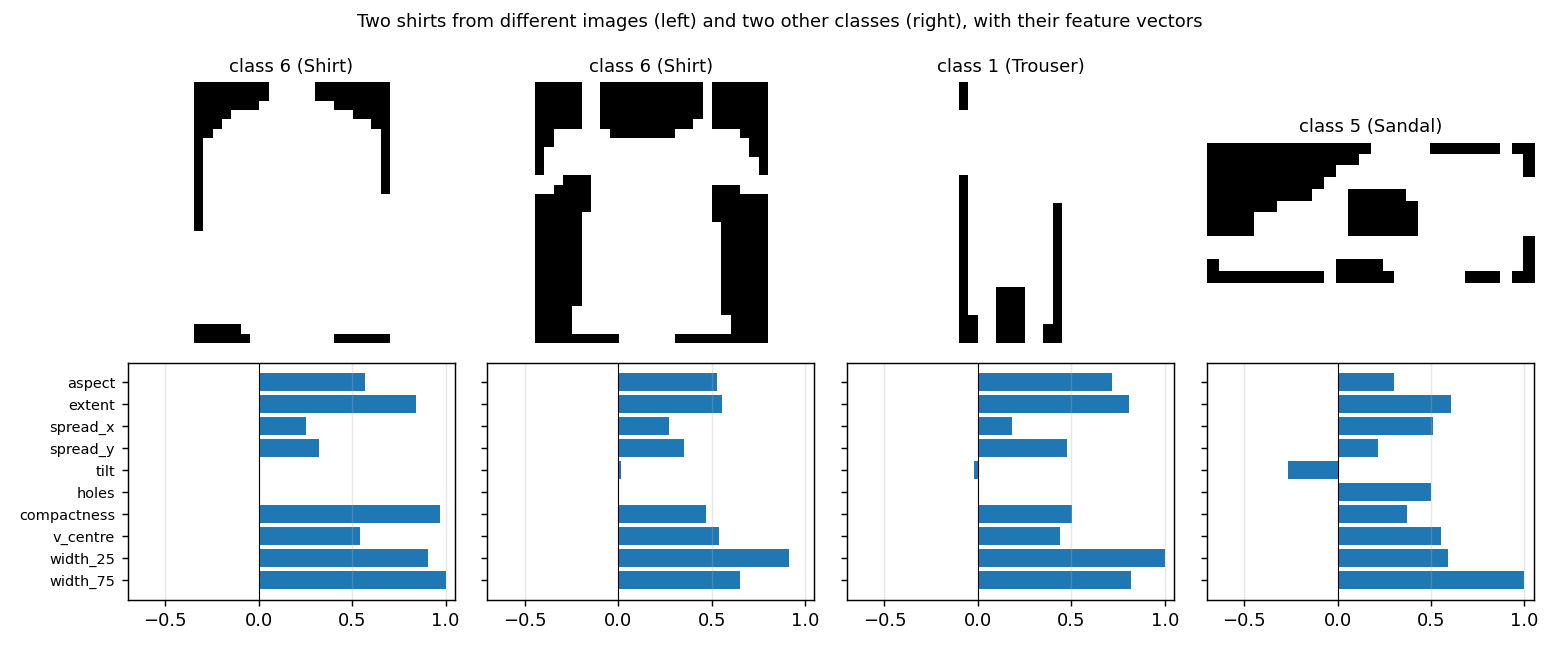
\includegraphics[width=\textwidth]{garment_examples.png}
    \caption{Two shirts from different images and two other classes, with
    their feature vectors.}
    \label{fig:garmentex}
\end{figure}

Both expectations are largely confirmed. The two shirts agree to within
$0.04$ on aspect, exactly on v\_centre and to within $0.01$ on width\_25, as
predicted. The trouser and the sandal differ by $0.42$ in aspect and by $0.25$
in tilt, which is a much larger gap than anything we see within a class. But
the shirts do \emph{not} agree on everything: their compactness is $0.97$
against $0.47$ and their extent $0.84$ against $0.56$, which is a far bigger
within-class difference than we expected. The reason is visible in the
figure: in shirt B the sleeves stand away from the body, so the silhouette has
deep notches under the arms, while in shirt A they do not. Both the fill
fraction and the length of the boundary change a lot as a result.

To make this precise we compared, for each feature, the average spread within
a class with the spread between class means. The ratio of the two says how
useful a feature is:

\begin{table}[H]
    \centering
    \small
    \begin{tabular}{lccccccccc}
        \toprule
        holes & width\_25 & spread\_x & aspect & tilt & spread\_y
        & v\_centre & extent & compact. & width\_75 \\
        \midrule
        6.5 & 4.3 & 4.1 & 4.0 & 3.4 & 2.8 & 2.5 & 2.1 & 1.6 & 1.1 \\
        \bottomrule
    \end{tabular}
    \caption{Between-class spread divided by within-class spread, largest
    first.}
\end{table}

The most discriminative features are the number of holes, which by itself
identifies bags, followed by width\_25, spread\_x, aspect and tilt. At the
other end, width\_75 has a ratio of only $1.1$, meaning it varies almost as
much inside a class as between classes, and compactness is not much better at
$1.6$. These are exactly the two features that disagreed between the two
shirts.

Running leave-one-out nearest neighbour on the standardised features
classifies \textbf{29 of the 50 segments correctly}, or $58\%$, against $10\%$
for guessing. Trousers and bags are recognised perfectly, $5/5$ and $3/3$,
while pullovers are never recognised, $0/3$.

\begin{figure}[H]
    \centering
    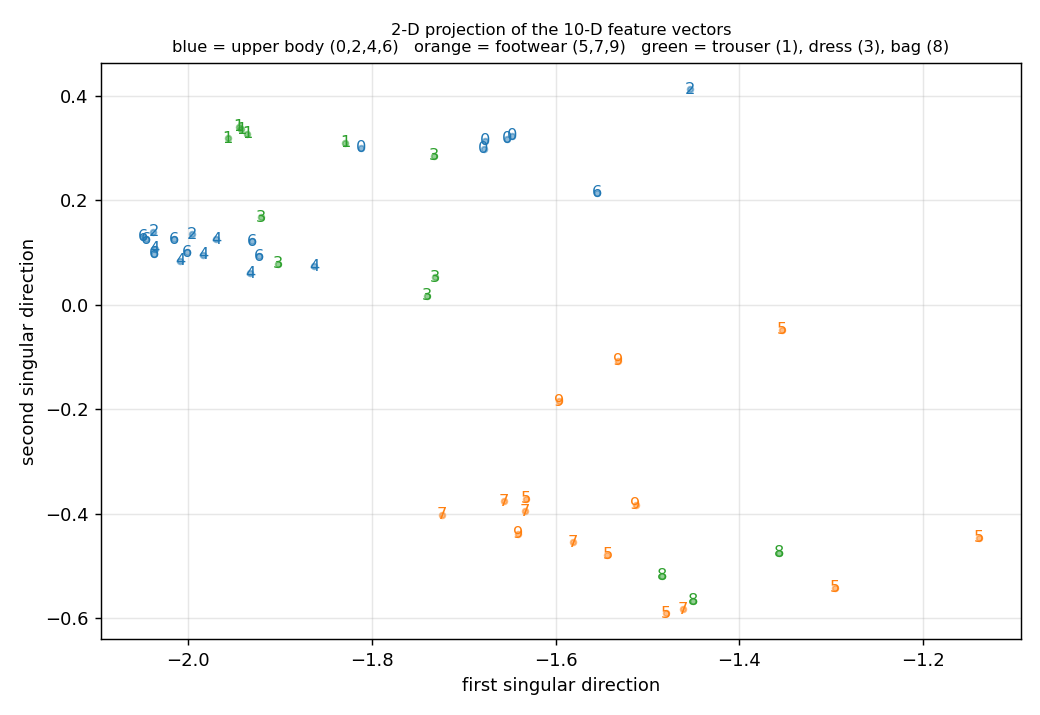
\includegraphics[width=0.85\textwidth]{garment_projection.png}
    \caption{The benchmark's two-dimensional projection of the feature
    vectors. The three families separate clearly, but the classes inside each
    family overlap.}
    \label{fig:garmentproj}
\end{figure}

The projection in Figure~\ref{fig:garmentproj} shows what is happening. The
upper-body garments form one tight cluster on the left, the footwear forms
another at the bottom, and trousers, dresses and bags sit apart from both.
The \emph{families} are well separated, but inside each family the classes are
piled on top of one another.

\begin{question}
Discuss at least one plausible failure mode: give an example of two garment
shapes that could obtain similar feature vectors, or one garment whose feature
vector could change substantially because of shape, scale, rotation,
segmentation error, or another relevant variation.
\end{question}

The clearest failure mode is the pair coat and shirt. Both are upper-body
garments with two sleeves and a straight hem, so their silhouettes are almost
the same, and every one of our features is computed from the silhouette alone.
The benchmark confirms this: three coats are classified as shirts and two
shirts as coats, the two largest confusions in the whole dataset. Taken as a
group, the four upper-body classes get only $11$ of $22$ right, and nine of
the eleven errors are to another class \emph{within} the group. Footwear
behaves the same way: $7$ of $15$ correct, and all eight errors stay inside
the footwear group. What actually distinguishes a coat from a shirt is the
front opening, the buttons and the texture of the fabric, none of which
survives in a binary mask, so this failure is a limitation of the input rather
than of our particular choice of features.

A second failure mode concerns rotation. None of our features is rotation
invariant, and two of them, tilt and aspect, would change a great deal if a
garment were laid down at a different angle. A sneaker photographed pointing
the other way would flip the sign of its tilt from $-0.27$ to $+0.27$ and
would then look, to the classifier, unlike any sneaker it has seen. The same
applies to segmentation errors: if the threshold from Assignment~1 clipped a
sleeve, the bounding box would shrink and aspect, extent and both width
features would all shift at once.

\begin{question}
If you were allowed to add or replace one feature after inspecting the
results, explain what you would change and what weakness in the current
representation you would try to address.
\end{question}

We would replace width\_75. It is the weakest feature we have, with a
between-class to within-class ratio of only $1.1$, so it carries almost no
information: nearly every garment is close to its widest at three quarters of
its height, whether it is a coat, a shirt or a sneaker.

In its place we would use the full row-width profile, resampled to a fixed
number of steps down the height and divided by the widest row. This is still
translation and scale invariant, but instead of one number at one height it
describes the whole outline, and it is the kind of detail that could separate
a coat from a shirt: a coat has roughly straight sides, whereas a shirt tapers
from the shoulders to the waist. Our current pair of width measurements
samples that profile at only two points and misses the shape in between. This
addresses the weakness that our features describe the silhouette only very
coarsely, which is what makes all four upper-body classes collapse into a
single cluster in Figure~\ref{fig:garmentproj}.


\end{document}

